\documentclass[aspectratio=169,11pt]{beamer}

% Build from this directory: latexmk -xelatex main.tex
% Local adaptation of the DIINF USACH course presentation style.
% All graphic dependencies live in this presentation's images/ directory.
\usetheme{Berlin}
\usecolortheme{seahorse}
\usefonttheme{professionalfonts}
\setbeamertemplate{headline}{}

\usepackage{iftex}
\ifPDFTeX
  \usepackage[utf8]{inputenc}
  \usepackage[T1]{fontenc}
  \usepackage[scaled=0.96]{helvet}
\else
  \usepackage{fontspec}
  \IfFontExistsTF{Noto Sans}
    {\setsansfont{Noto Sans}}
    {\setsansfont{TeX Gyre Heros}}
\fi
\renewcommand{\familydefault}{\sfdefault}
\usepackage[provide=*]{babel}
\babelprovide[main,import]{english}
\usepackage{amsmath}
\usepackage{graphicx}
\usepackage{booktabs}
\usepackage{tabularx}
\usepackage{tikz}
\usetikzlibrary{positioning,arrows.meta,calc}
\graphicspath{{images/}}
\newcolumntype{L}[1]{>{\raggedright\arraybackslash}p{#1}}
\newcolumntype{Y}{>{\raggedright\arraybackslash}X}

% Colores del sitio DIINF: wp-content/uploads/elementor/css/post-6.css.
\definecolor{diinfTurquesa}{HTML}{00A499}
\definecolor{diinfGris}{HTML}{394049}
\definecolor{diinfVioleta}{HTML}{7C3581}
\definecolor{diinfGrisClaro}{HTML}{EBEBEB}
% Tonos de apoyo para contraste y superficies de lectura.
\definecolor{diinfTextoSecundario}{HTML}{59636D}
\colorlet{diinfTurquesaOscuro}{diinfTurquesa!65!black}
\colorlet{diinfFondo}{diinfGrisClaro!45!white}
\colorlet{diinfFondoTurquesa}{diinfTurquesa!8!white}

\setbeamercolor{normal text}{fg=diinfGris,bg=white}
\setbeamercolor{title}{fg=diinfTurquesaOscuro}
\setbeamercolor{frametitle}{fg=diinfGris,bg=diinfFondo}
\setbeamercolor{frametitle rule}{bg=diinfTurquesa}
\setbeamercolor{structure}{fg=diinfTurquesaOscuro}
\setbeamercolor{item}{fg=diinfTurquesa}
\setbeamercolor{alerted text}{fg=diinfVioleta}
\setbeamercolor{block title}{fg=white,bg=diinfTurquesaOscuro}
\setbeamercolor{block body}{fg=diinfGris,bg=diinfFondoTurquesa}
\setbeamercolor{block title alerted}{fg=white,bg=diinfVioleta}
\setbeamercolor{block body alerted}{fg=diinfGris,bg=diinfVioleta!6!white}
\setbeamercolor{block title example}{fg=white,bg=diinfGris}
\setbeamercolor{block body example}{fg=diinfGris,bg=diinfFondo}
\setbeamercolor{footline}{fg=diinfTextoSecundario,bg=white}
\setbeamerfont{frametitle}{series=\bfseries,size=\Large}
\setbeamerfont{title}{series=\bfseries,size=\LARGE}
\setbeamerfont{block title}{series=\bfseries,size=\normalsize}
\setbeamerfont{footline}{size=\scriptsize}
\setbeamertemplate{navigation symbols}{}
\setbeamertemplate{blocks}[rounded][shadow=false]
\setbeamertemplate{frametitle}{%
  \nointerlineskip
  \begin{beamercolorbox}[wd=\paperwidth,ht=0.78cm,dp=0.22cm,
    leftskip=0.68cm,rightskip=0.55cm]{frametitle}
    \usebeamerfont{frametitle}\insertframetitle
  \end{beamercolorbox}%
  \nointerlineskip
  \begin{beamercolorbox}[wd=\paperwidth,ht=0.055cm,dp=0cm]{frametitle rule}
  \end{beamercolorbox}%
}
\setbeamertemplate{footline}{%
  \leavevmode
  \hbox{%
    \begin{beamercolorbox}[wd=0.68\paperwidth,ht=0.49cm,dp=0.16cm,
      leftskip=0.62cm]{footline}
      \usebeamerfont{footline}\insertshorttitle
      \ifx\insertsectionhead\empty\else
        \enspace\textcolor{diinfTurquesa}{\textbullet}\enspace\insertsectionhead
      \fi
    \end{beamercolorbox}%
    \begin{beamercolorbox}[wd=0.20\paperwidth,ht=0.49cm,dp=0.16cm,
      center]{footline}
      \raisebox{-0.07cm}{
\includegraphics[width=1.85cm]{diinf-usach-logo.png}}
    \end{beamercolorbox}%
    \begin{beamercolorbox}[wd=0.12\paperwidth,ht=0.49cm,dp=0.16cm,
      rightskip=0.62cm]{footline}
      \hfill\usebeamerfont{footline}\insertframenumber\,/\,\inserttotalframenumber
    \end{beamercolorbox}%
  }%
}
\setbeamersize{text margin left=0.68cm,text margin right=0.68cm}
\setlength{\leftmargini}{1.25em}
\setlength{\leftmarginii}{1.1em}
\setbeamertemplate{itemize items}[circle]
\setbeamertemplate{enumerate items}[circle]
\setbeamerfont{itemize/enumerate body}{size=\normalsize}
\setbeamerfont{itemize/enumerate subbody}{size=\small}
\setlength{\emergencystretch}{1em}

\newcommand{\diinflogo}{
\includegraphics[width=3.8cm]{diinf-usach-logo.png}}
\newcommand{\etiqueta}[2][diinfTurquesaOscuro]{%
  \tikz[baseline=(tag.base)]{\node[draw=#1,text=#1,rounded corners=2pt,
    inner xsep=6pt,inner ysep=3pt,font=\bfseries\footnotesize]
    (tag) {#2};}%
}
\newcommand{\idea}[1]{%
  \begin{block}{}\centering\large #1\end{block}%
}
\newcommand{\fuente}[1]{%
  \par\vspace{0.45em}{\scriptsize\color{diinfTextoSecundario}#1\par}%
}

\newcommand{\portada}{%
  \begin{frame}[plain,noframenumbering]
    \begin{tikzpicture}[remember picture,overlay]
      \fill[diinfTurquesa] (current page.south west)
        rectangle ([xshift=0.42cm]current page.north west);
      \fill[diinfTurquesa!12] ([xshift=0.42cm]current page.south west)
        rectangle ([xshift=0.62cm]current page.north west);
      \node[anchor=north east] at
        ([xshift=-0.76cm,yshift=-0.58cm]current page.north east) {\diinflogo};
      \node[anchor=west,text width=13cm,align=left] at
        ([xshift=1.28cm,yshift=0.35cm]current page.west) {
        {\fontsize{28}{33}\selectfont\bfseries\color{diinfGris}\inserttitle}\\[0.50em]
        {\fontsize{21}{26}\selectfont\bfseries\color{diinfTurquesaOscuro}\insertsubtitle}
      };
      \draw[diinfVioleta,line width=1pt]
        ([xshift=1.28cm,yshift=-1.35cm]current page.west) --
        ([xshift=7.5cm,yshift=-1.35cm]current page.west);
      \node[anchor=south west,text width=12.8cm,align=left] at
        ([xshift=1.28cm,yshift=0.65cm]current page.south west) {
        {\normalsize\bfseries\insertinstitute}\\[0.45em]
        {\small\color{diinfTextoSecundario}\insertdate}
      };
    \end{tikzpicture}
  \end{frame}%
}

\AtBeginSection[]{%
  \begin{frame}[plain,noframenumbering]
    \begin{tikzpicture}[remember picture,overlay]
      \fill[diinfTurquesa] (current page.south west)
        rectangle ([xshift=0.34cm]current page.north west);
      \fill[diinfTurquesa!12] ([xshift=0.34cm]current page.south west)
        rectangle ([xshift=0.50cm]current page.north west);
      \node[anchor=north east] at
        ([xshift=-0.72cm,yshift=-0.52cm]current page.north east) {\diinflogo};
      \node[anchor=west,text width=13.6cm,align=left] at
        ([xshift=1.12cm,yshift=0.35cm]current page.west) {
        {\large\color{diinfTextoSecundario}\insertshorttitle}\\[0.85em]
        {\fontsize{25}{30}\selectfont\bfseries\color{diinfGris}\insertsectionhead}
      };
      \draw[diinfVioleta,line width=0.7pt]
        ([xshift=1.12cm,yshift=-1.25cm]current page.west) --
        ([xshift=-0.75cm,yshift=-1.25cm]current page.east);
      \node[anchor=south east,text=diinfTurquesa!20,
        font=\fontsize{54}{54}\selectfont\bfseries] at
        ([xshift=-0.72cm,yshift=0.45cm]current page.south east) {0\thesection};
    \end{tikzpicture}
  \end{frame}%
}

\usepackage{fancyhdr}
\usepackage{graphicx}
\usepackage{appendixnumberbeamer}
\usetikzlibrary{fit,backgrounds}
\setbeameroption{hide notes}
% Keep sections in the footer without adding separate section title slides.
\AtBeginSection[]{}
\setbeamerfont{itemize/enumerate body}{size=\small}

\title[Proyecto RL]{Proyecto RL}
\subtitle{Procesamiento de tareas en red satelital}
\author[Camilo J. Rojas Milla]{Camilo José Rojas Milla}
\institute{}
\date{}
\hypersetup{
  pdftitle={Proyecto RL: procesamiento de tareas en red satelital},
  pdfauthor={Camilo Jose Rojas Milla},
  pdfsubject={Ambiente de aprendizaje por refuerzo para procesamiento satelital},
  pdfkeywords={Aprendizaje por refuerzo, Gymnasium, redes satelitales, procesamiento de tareas},
  colorlinks=true,urlcolor=diinfTurquesaOscuro,linkcolor=diinfTextoSecundario
}

\newcommand{\trajectorycell}[4]{%
  \begingroup
  \setlength{\fboxsep}{0pt}%
  \fbox{%
  \begin{minipage}[t][3.5cm][c]{6cm}
    \centering
    \vspace{0.1cm}
    {\scriptsize\textbf{#2}}\\[-0.5em]
    {\tiny #3}\\[-0.6em]
    {\tiny #4}\\[0.1em]
    #1
  \end{minipage}}%
  \endgroup
}

\newcommand{\source}[1]{\fuente{#1}}
\newcommand{\paperfigure}{\source{Source: current paper.}}
\newcommand{\takeaway}[1]{\vspace{0.25em}\idea{#1}}
\newenvironment{points}{\begin{itemize}\setlength\itemsep{0.8em}}{\end{itemize}}
\newenvironment{projectpoints}{\begin{itemize}\setlength\itemsep{0.55em}}{\end{itemize}}
% Replace each placeholder with \includegraphics when its figure is ready.
\newcommand{\figurapendiente}[1]{%
  \begin{tikzpicture}
    \node[draw=diinfGris!25,dashed,rounded corners=3pt,
      fill=diinfFondo!50,minimum height=4.6cm,
      text width=\dimexpr\linewidth-16pt\relax,inner sep=7pt,
      align=center,text=diinfTextoSecundario,font=\scriptsize]
      {Figura por incorporar\\[0.6em]#1};
  \end{tikzpicture}%
}
\newcommand{\stat}[3]{%
  \begin{minipage}[t]{#1}\centering
    {\fontsize{30}{34}\selectfont\bfseries\color{diinfTurquesaOscuro}#2\par}
    \vspace{0.45em}{\normalsize #3\par}
  \end{minipage}%
}
\tikzset{
  flowbox/.style={draw=diinfTurquesaOscuro,fill=diinfFondoTurquesa,
    rounded corners=3pt,align=center,minimum height=1.05cm,
    text width=2.65cm,inner sep=6pt,font=\small},
  flowarrow/.style={-{Latex[length=2.5mm]},thick,diinfTurquesaOscuro},
  mutedbox/.style={flowbox,draw=diinfGris!50,fill=diinfFondo},
  purplebox/.style={flowbox,draw=diinfVioleta,fill=diinfVioleta!7}
}

% Shared RL diagram: images replace the agent and environment boxes.
\newcommand{\diagramarl}{%
  \resizebox{\linewidth}{!}{%
    \begin{tikzpicture}[font=\normalsize]
      \path[use as bounding box] (-2.15,-2.25) rectangle (2.15,2.25);
      \node[inner sep=3pt] (agente) at (0,1.35)
        {
\includegraphics[width=1.15cm]{images/cerebro.png}};
      \node[inner sep=3pt] (ambiente) at (0,-1.25)
        {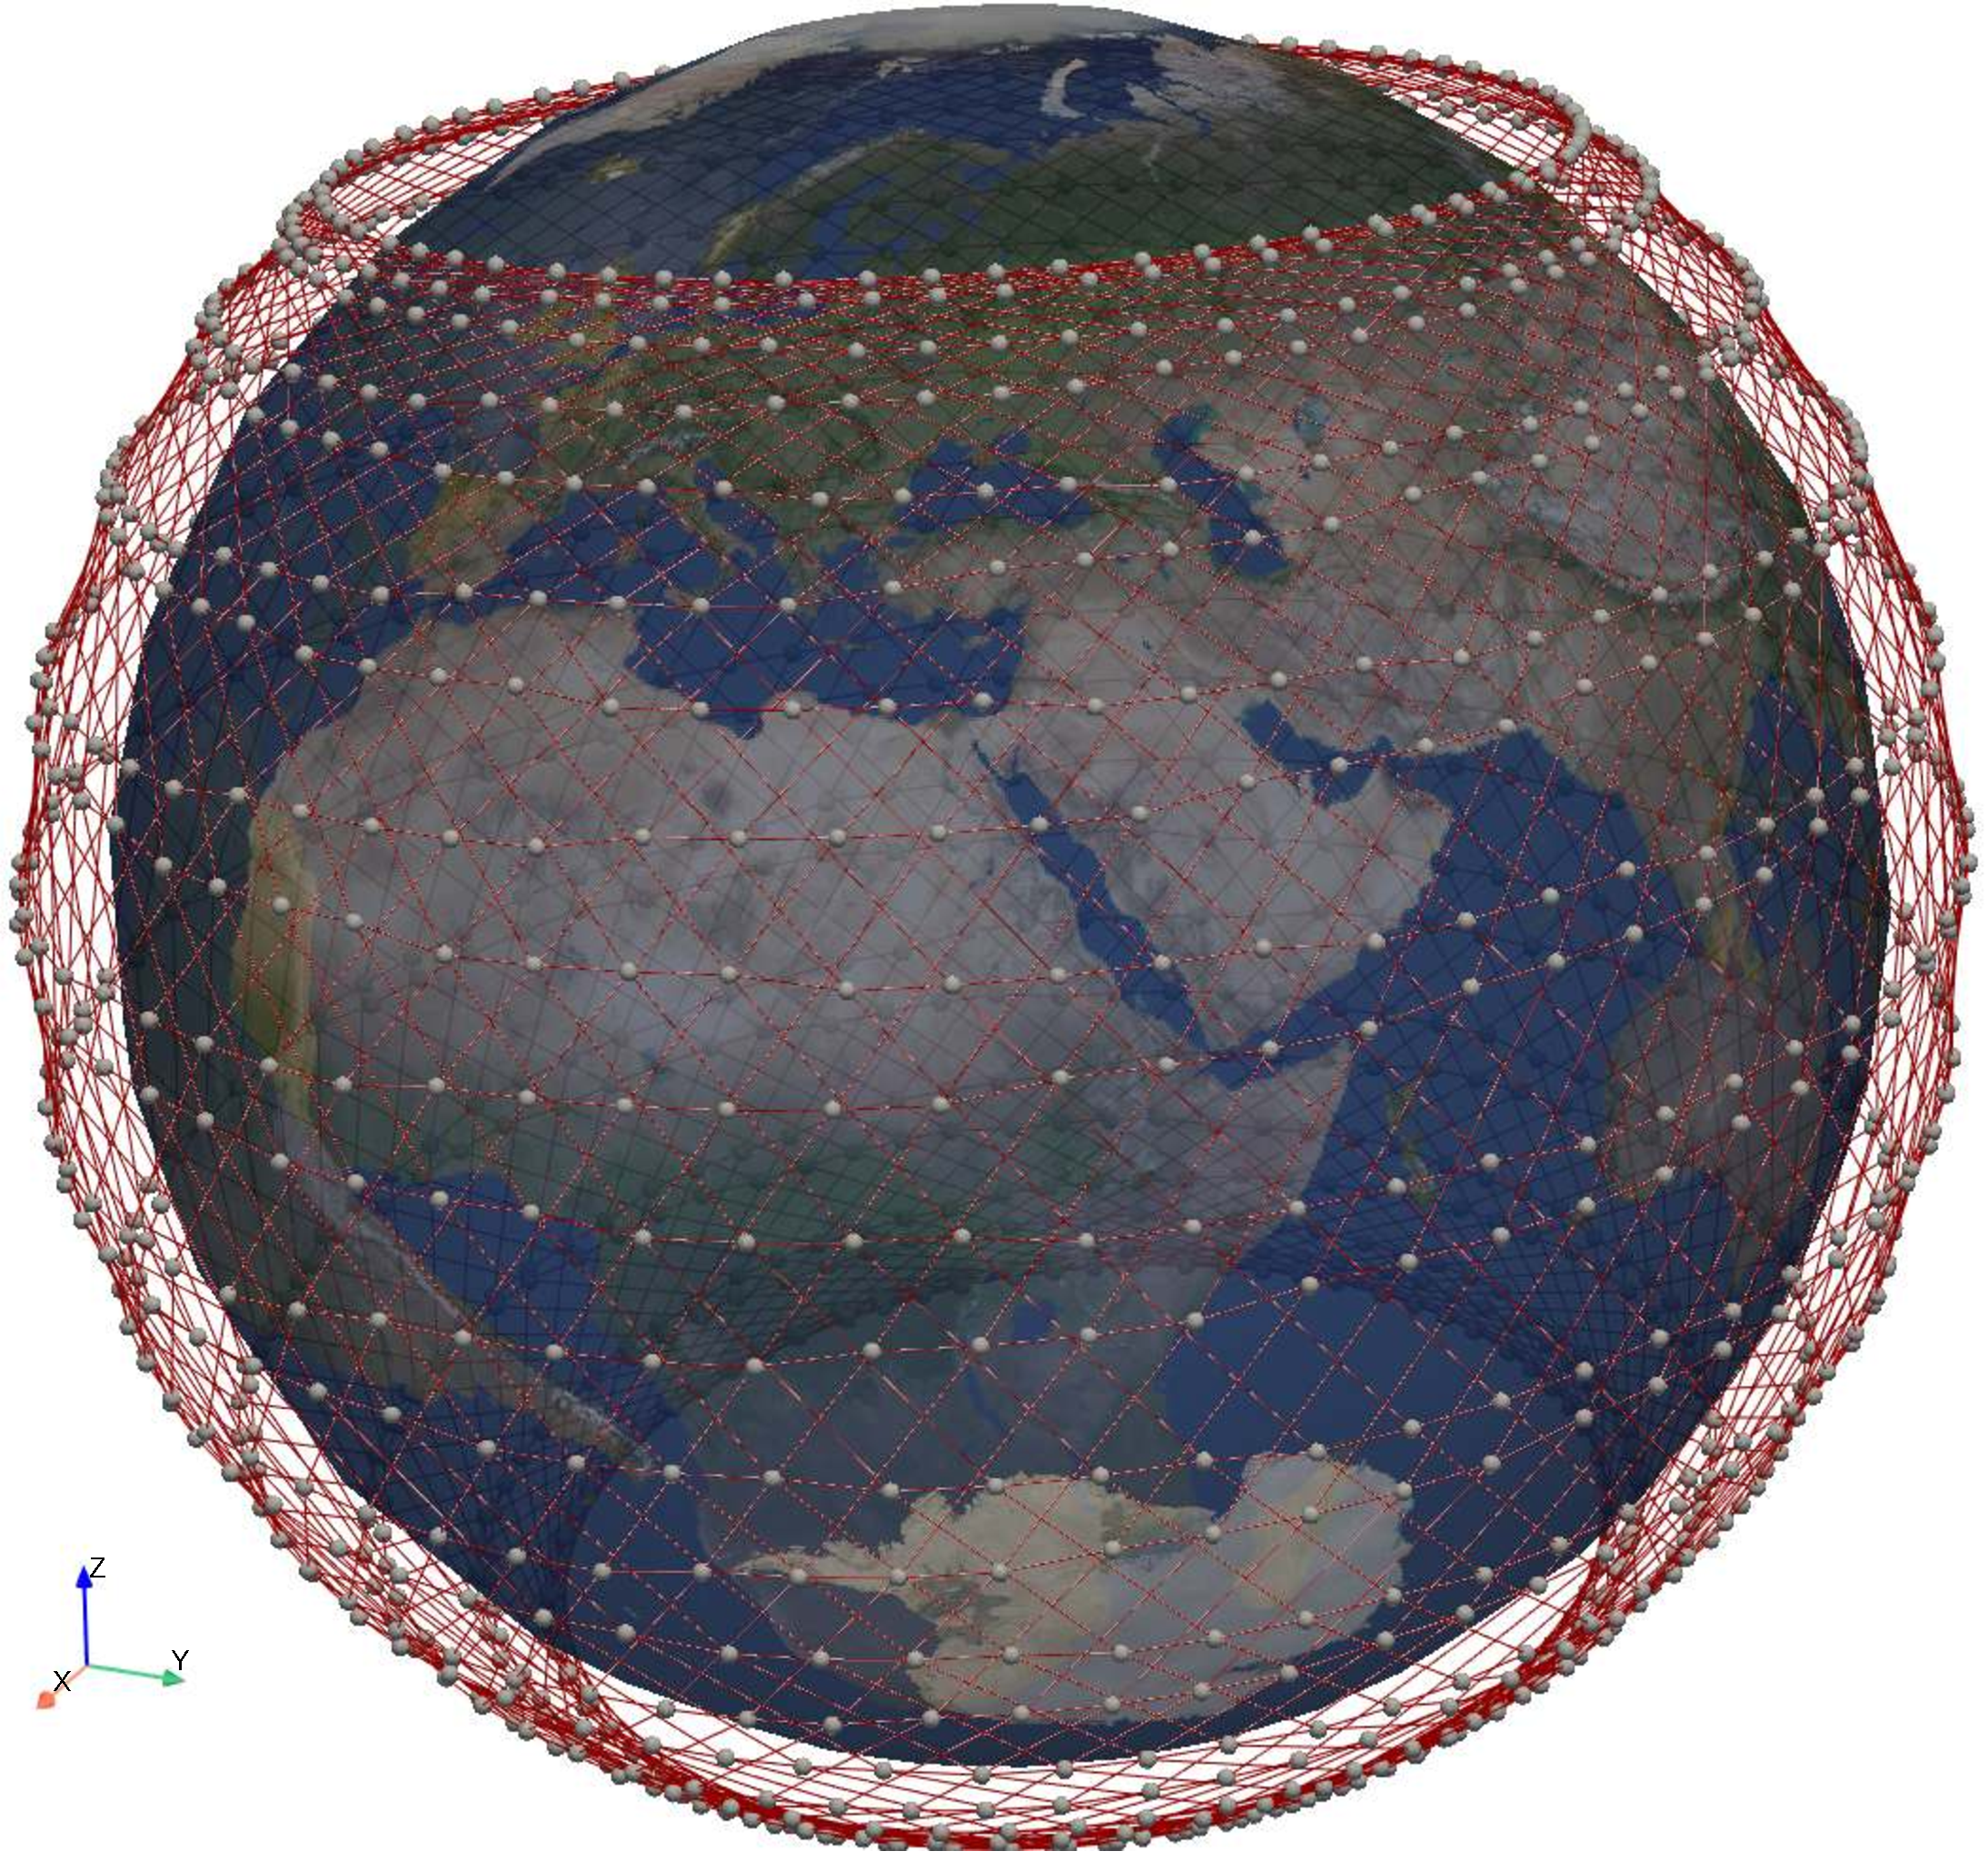
\includegraphics[width=1.8cm]{images/starlink.pdf}};
      \draw[flowarrow,diinfVioleta]
        (agente.east) -- (1.55,1.35)
        -- node[right,inner sep=4pt] {$A_t$} (1.55,-1.25)
        -- (ambiente.east);
      \draw[flowarrow]
        (ambiente.west) -- (-1.55,-1.25)
        -- node[left,inner sep=4pt] {$S_t$} (-1.55,1.35)
        -- (agente.west);
      \draw[flowarrow]
        (ambiente.north) -- node[right,inner sep=4pt] {$r_t$} (agente.south);
    \end{tikzpicture}%
  }%
}

\begin{document}

% Portada.
\begin{frame}[plain,noframenumbering]
  \begin{tikzpicture}[remember picture,overlay]
    \fill[diinfTurquesa] (current page.south west)
      rectangle ([xshift=0.42cm]current page.north west);
    \fill[diinfTurquesa!12] ([xshift=0.42cm]current page.south west)
      rectangle ([xshift=0.62cm]current page.north west);
    \node[anchor=north east] at
      ([xshift=-0.76cm,yshift=-0.58cm]current page.north east) {\diinflogo};
    \node[anchor=north west,text width=13.6cm,align=left] at
      ([xshift=1.15cm,yshift=-2.15cm]current page.north west) {
      {\fontsize{27}{33}\selectfont\bfseries\color{diinfGris}
        Proyecto RL \\[0.65em]
        Procesamiento de tareas\\
        en red satelital}\par
    };
    \draw[diinfVioleta,line width=1pt]
      ([xshift=1.15cm,yshift=2.6cm]current page.south west) --
      ([xshift=7.5cm,yshift=2.6cm]current page.south west);
    \node[anchor=south west,text width=13.3cm,align=left] at
      ([xshift=1.15cm,yshift=0.75cm]current page.south west) {
      {\large\bfseries\insertauthor}
    };
  \end{tikzpicture}
\end{frame}

\section{Introducción}
\begin{frame}{Introducción}
  \small
  \begin{columns}[c,onlytextwidth]
    \column{0.55\textwidth}
      % Keep the original diagram on the first content slide.
      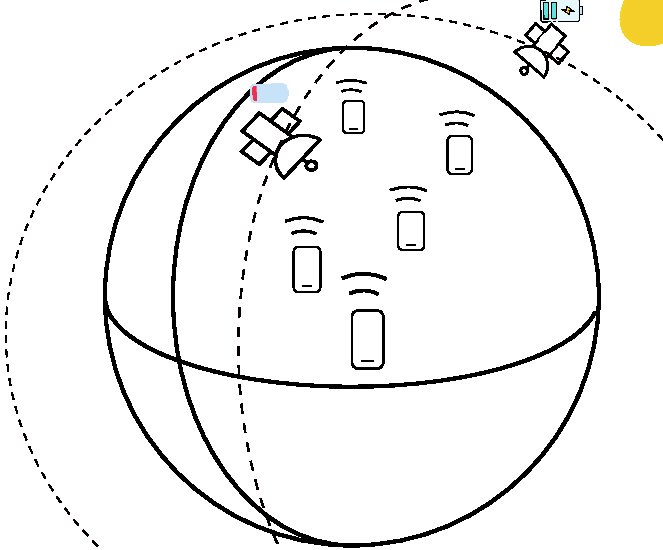
\includegraphics[width=\linewidth]{images/constellation.pdf}
    \column{0.42\textwidth}
      \begin{block}{Objetivo}
        Decidir qué satélites estarán disponibles para procesar
        tareas generadas por usuarios en tierra.
      \end{block}
      \vspace{0.6em}
      \textbf{Ambiente de aprendizaje}
      \begin{projectpoints}
        \item Implementación en \textbf{Python} con \textbf{Gymnasium}.
        \item Datos del ambiente disponibles en cada paso $\Delta t$.
        \item Decisión: activar o desactivar el procesamiento en los satélites.
      \end{projectpoints}
  \end{columns}
\end{frame}

\section{Ambiente}
\begin{frame}{Ambiente: segmento espacial y terrestre}
  \small
  \begin{columns}[T,onlytextwidth]
    \column{0.5\textwidth}

        \textbf{Segmento espacial}
          \begin{itemize}
            \setlength\itemsep{0.25em}
            \item Satélites en órbitas \textbf{LEO}.
            \item Estado \textbf{activo}: procesa tareas;
              \textbf{pasivo}: no procesa.
            \item El ambiente entrega variables operacionales cuando
              hay usuarios en línea de vista.
          \end{itemize}


    \column{0.5\textwidth}
             \textbf{Segmento terrestre}
          \begin{itemize}
            \setlength\itemsep{0.25em}
            \item Los usuarios generan tareas $\tau$ aleatoriamente; una nueva solo cuando la anterior se completa o falla.
            \item \textbf{Éxito:} subir la tarea al \textbf{satélite activo más cercano} en línea de vista. \textbf{Fallo:} transcurren $R_{\tau}$ segundos sin completarse.
          \end{itemize}

  \end{columns}
  \centering
  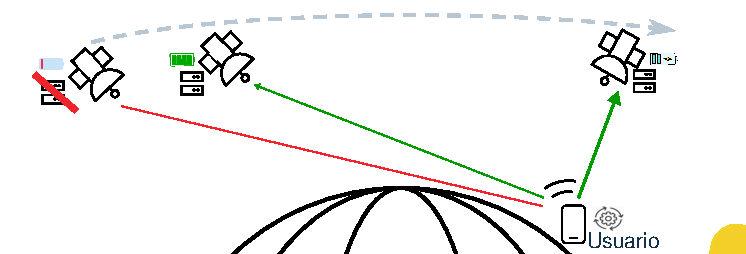
\includegraphics[width=0.75\textwidth]{images/segmentos.pdf}
\end{frame}

\section{Restricciones}
\begin{frame}{Restricciones: batería y disponibilidad}
  \small
  \begin{columns}[T,onlytextwidth]
    \column{0.50\textwidth}
      \begin{projectpoints}
        \item \textbf{Día orbital:} los paneles solares cargan la batería
          al recibir luz del Sol.
        \item \textbf{Noche orbital:} la Tierra bloquea la luz solar y
          la batería se descarga. Ciclos orbitales de unos \textbf{90 minutos}.
        \item \textbf{Estado activo:} acelera la descarga;
          procesar una tarea añade consumo.
      \end{projectpoints}
      \vspace{0.4em}
      \begin{alertblock}{Límite de batería}
        Al alcanzar la capacidad límite, se suspende el procesamiento
        hasta recargar la batería.
      \end{alertblock}
    \column{0.47\textwidth}
      \centering
      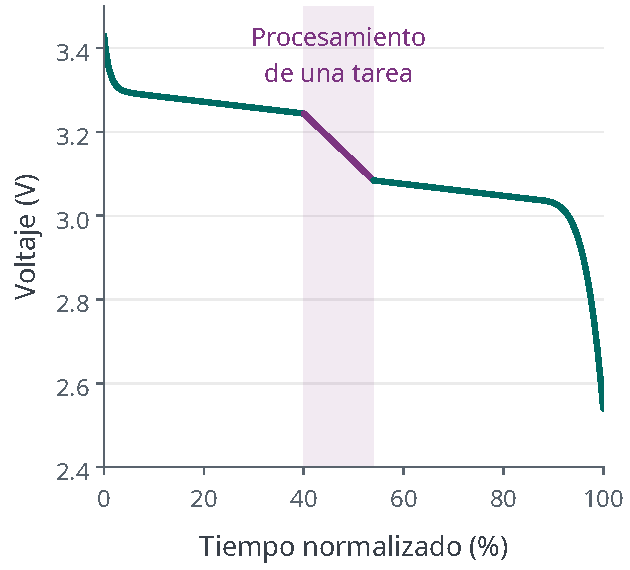
\includegraphics[width=\linewidth]{images/curva_voltaje.pdf}
      \par\vspace{0.3em}
      {\scriptsize\color{diinfTextoSecundario}Curva esquemática de descarga.}
  \end{columns}
\end{frame}

\section{Recompensa, estado y acción}
\begin{frame}{Recompensa, estado y acción: variables del estado}
  \small
  \begin{columns}[T,onlytextwidth]
    \column{0.65\textwidth}
      Para cada instante $t$ y satélite $s$, el estado puede incluir:
      \vspace{0.5em}

      {\renewcommand{\arraystretch}{1.22}
      \begin{tabularx}{\linewidth}{@{}lY@{}}
        \toprule
        \textbf{Variable} & \textbf{Información del ambiente} \\
        \midrule
        $u_s$ & Número de usuarios en línea de vista. \\
        $U_s$ & Identidad de los usuarios. \\
        $T_s$ & Largo de las tareas pendientes por usuario. \\
        $R_s$ & Tiempo restante antes de que cada tarea falle. \\
        $D_s$ & Distancia a los usuarios en línea de vista. \\
        $P_s,\ L_s$ & Posición cartesiana y geográfica del satélite. \\
        $V_s$ & Vector de velocidad del satélite\\
        $c_s,\ e_s$ & Carga de batería y estado: cargando o descargando. \\
        \bottomrule
      \end{tabularx}}
      \vspace{0.5em}

      {\footnotesize
        $U_s, T_s, R_s, D_s$: vectores de dimensión $u_s\times 1$.\\[0.25em]
        $P_s=(x_s,y_s,z_s)$;\quad
        $L_s=(\mathrm{lat}_s,\mathrm{lon}_s,h_s)$.\par}
    \column{0.31\textwidth}
      \diagramarl
  \end{columns}
\end{frame}

\begin{frame}{Recompensa, estado y acción: decisión y evaluación}
  \small
  \begin{columns}[T,onlytextwidth]
    \column{0.65\textwidth}
      \begin{block}{Acción $A$}
        Vector de dimensión $S\times 1$, con una decisión por satélite:
        \[
          A=(a_1,\ldots,a_S),\qquad a_s\in\{0,1\}.
        \]
        \textbf{1:} activar el procesamiento.\quad
        \textbf{0:} desactivarlo.
      \end{block}
      \vspace{0.4em}
      \begin{block}{Recompensa $r$}
        Suma las tareas completadas exitosamente y resta las fallidas:
        \[
          r=N_{\text{exitosas}}-N_{\text{fallidas}}.
        \]
      \end{block}
      \vspace{0.3em}
      $S$ es el número de satélites de la constelación.
    \column{0.31\textwidth}
      \diagramarl
  \end{columns}
\end{frame}

\section{Entrenamiento}
\begin{frame}{Entrenamiento: episodios e interacción}
  \small
  \begin{columns}[T,onlytextwidth]
    \column{0.65\textwidth}
      \begin{projectpoints}
        \item El entrenamiento se organiza en \textbf{episodios de duración $T$},
          compuestos por sucesivos pasos $\Delta t$.
        \item La constelación mantiene fijo su número de satélites $S$
          durante cada episodio.
        \item Los usuarios y las tareas pueden aparecer o desaparecer;
          las tareas pueden tener distintos largos.
      \end{projectpoints}
      \vspace{0.4em}
      \begin{block}{En cada instante $t$}
        Observar las variables del ambiente, elegir la acción $A$,
        aplicarla a los satélites y evaluar el resultado con la recompensa $r$.
      \end{block}
    \column{0.31\textwidth}
         $$\mathbb{T} = \{t_0, t_1 \ldots T\}$$
         $$t_{n+1} \leftarrow t_n + \Delta t$$
      \diagramarl
  \end{columns}
\end{frame}




% \begin{frame}[c]{Cierre}
%   \centering
%   {\LARGE\bfseries\color{diinfTurquesaOscuro}Gracias por su Atención!\par}
%   \vspace{0.8em}
%   {\large Esperamos Trabajar Contigo.\par}
%   \vspace{2em}
%   {\Large\bfseries\insertauthor\par}
%   \vspace{0.5em}
%   {\large\href{mailto:camilo.rojas.m@usach.cl}{camilo.rojas.m@usach.cl}\par}
% \end{frame}

\end{document}
